\chapter{Analisi Comparativa delle Tecnologie e degli Strumenti}
\label{ch:tecnologie_strumenti}

Lo sviluppo di un sistema software innovativo, specialmente in un contesto \gls{agile} come quello di una startup, richiede un'attenta valutazione delle tecnologie disponibili. Ogni scelta architetturale implica un compromesso tra \textit{performance}, costi, tempi di sviluppo e manutenibilità futura. Questo capitolo non si limita a elencare gli strumenti adottati per la realizzazione del prototipo, ma si propone di analizzare criticamente il panorama tecnologico per ciascun dominio problematico affrontato.

L'analisi seguirà una struttura sistematica per ogni componente dell'architettura:
\begin{enumerate}
    \item \textbf{Definizione del problema}: si delineerà la sfida tecnica o funzionale da risolvere.
    \item \textbf{Analisi delle alternative}: si esamineranno le principali tecnologie e approcci disponibili sul mercato per affrontare tale sfida, valutandone pro e contro.
    \item \textbf{Soluzione adottata e motivazioni}: si presenterà la scelta effettuata, giustificandola non solo in base a meriti tecnici intrinseci, ma anche in relazione al contesto specifico del progetto, ovvero l'ecosistema di Devess, gli obiettivi della tesi e i vincoli operativi.
\end{enumerate}

% --------------------------------------------------------------------
\section{Architettura del Back-end e Comunicazione API}
\label{sec:backend_analysis}

\subsection{Definizione del problema}
Il \gls{backend} rappresenta il nucleo logico dell'applicazione. La sfida consiste nel creare un servizio che abbia la duplice responsabilità di esporre un'interfaccia \gls{api} sicura e performante per il \gls{frontend} e di orchestrare le complesse interazioni con i modelli linguistici e le fonti dati esterne. La sua progettazione è cruciale per la reattività e la scalabilità dell'intero sistema, specialmente dovendo gestire chiamate asincrone a lunga attesa verso servizi di terze parti come gli \gls{llm}.

\subsection{Analisi delle alternative}
La scelta del \gls{framework} e del linguaggio di programmazione per il \gls{backend} ha considerato tre principali candidati:

\begin{itemize}
    \item \textbf{Python con Django/Flask}: Python è il linguaggio d'elezione per il \textit{machine learning} e l'analisi dati. \textbf{Django} è un \gls{framework} "\textit{batteries-included}", robusto e maturo, ideale per progetti complessi con requisiti ben definiti. \textbf{Flask} è un \textit{micro-framework} minimale e flessibile, che lascia massima libertà allo sviluppatore. Tuttavia, entrambi richiedono configurazioni aggiuntive per una gestione efficiente della concorrenza asincrona, fondamentale per il nostro caso d'uso.
    
    \item \textbf{Node.js con Express.js/NestJS}: L'ecosistema JavaScript/TypeScript con Node.js è rinomato per il suo modello di \textit{I/O non bloccante}, che lo rende eccezionalmente performante per applicazioni \textit{real-time} e \textit{API-intensive}. \textbf{Express.js} è il \gls{framework} minimale di riferimento, mentre \textbf{NestJS} offre una struttura più opinionata e scalabile, ispirata ad Angular. Sebbene performante, l'ecosistema di Node.js per l'analisi dati e l'interazione scientifica non eguaglia ancora la maturità e la ricchezza di quello Python.
    
    \item \textbf{Python con FastAPI}: \textbf{FastAPI} è un \gls{framework} moderno che unisce la semplicità di Flask con \textit{performance} paragonabili a quelle di Node.js, grazie al supporto nativo per la programmazione asincrona (tramite ASGI). Offre inoltre vantaggi unici come la validazione dei dati basata sui \textit{type hint} di Python tramite Pydantic e la generazione automatica di documentazione interattiva (\textit{Swagger UI}), accelerando drasticamente il ciclo di sviluppo e test delle \gls{api}.
\end{itemize}

\subsection{Soluzione adottata e motivazioni}
La scelta è ricaduta su \textbf{Python} e sul \gls{framework} \textbf{FastAPI}. Le motivazioni sono strategiche e tecniche:
\begin{enumerate}
    \item \textbf{Ecosistema Python}: La necessità di integrare librerie di analisi dati come Pandas e di interagire fluidamente con \gls{framework} di orchestrazione \gls{llm} (come \gls{langchain}) ha reso Python la scelta più naturale e produttiva.
    \item \textbf{\textit{Performance} Asincrone}: FastAPI gestisce nativamente le operazioni asincrone. Questo è un requisito non negoziabile, in quanto il \gls{backend} deve attendere le risposte dall'\gls{llm} senza bloccare altre richieste concorrenti.
    \item \textbf{Produttività dello Sviluppatore}: La validazione automatica di Pydantic e la documentazione OpenAPI riducono il codice ripetitivo e il rischio di errori.
    \item \textbf{Coerenza Aziendale}: Python è già ampiamente utilizzato nell'azienda, il che rende la manutenibilità futura più facile e immediata, allineandosi alle competenze interne.
\end{enumerate}
%-------

\section{Selezione del Modello Linguistico}
\label{sec:llm_selection}

\subsection{Definizione del problema}
La scelta del \gls{llm} è il fulcro del sistema intelligente. Il problema non è selezionare un modello qualsiasi, ma individuare quello le cui capacità si allineano meglio ai requisiti specifici del progetto: non solo comprendere e generare linguaggio naturale, ma anche seguire istruzioni complesse, invocare strumenti esterni in modo affidabile e, soprattutto, analizzare dati strutturati forniti in formati comuni come il \gls{csv}. La scelta deve bilanciare \textit{performance} di ragionamento, costi operativi e facilità di integrazione.

\subsection{Analisi delle alternative}
Sono stati presi in considerazione i principali attori del mercato dei modelli linguistici:
\begin{itemize}
    \item \textbf{Modelli OpenAI (famiglia GPT)}: Rappresentano lo stato dell'arte per molteplici compiti di ragionamento generale. La loro \gls{api}, con la funzionalità di \textit{Function Calling}, è matura e ben documentata. Tuttavia, la loro capacità di analizzare direttamente file di dati strutturati può richiedere passaggi intermedi di pre-elaborazione.
    
    \item \textbf{Modelli Google (famiglia Gemini)}: Sono potenti alternative multimodali con un forte ecosistema alle spalle. Al momento della valutazione, le loro capacità di \textit{tool-calling} erano in rapida evoluzione ma potenzialmente meno consolidate rispetto ai concorrenti diretti per questo specifico caso d'uso.
    
    \item \textbf{Modelli Open-Source (es. Llama, Mixtral)}: Offrono il vantaggio del pieno controllo e dell'assenza di costi per \gls{api}, consentendo anche un \textit{fine-tuning} spinto. Di contro, richiedono un notevole onere infrastrutturale per l'\textit{hosting}, la gestione e la scalabilità. Inoltre, le loro capacità di seguire catene di ragionamento complesse e di usare strumenti in modo affidabile, sebbene in costante miglioramento, spesso non raggiungono ancora la robustezza dei migliori modelli proprietari.
\end{itemize}

\subsection{Soluzione adottata e motivazioni}
È stato scelto un modello della famiglia \textbf{Claude 4 di Anthropic}. Le ragioni di questa decisione sono strettamente legate ai requisiti funzionali del prototipo:
\begin{itemize}
    \item \textbf{Capacità di Analisi Dati}: I modelli Claude hanno dimostrato una capacità superiore nell'analizzare e interpretare direttamente il contenuto di file con dati strutturati, come il \gls{csv}, questa abilità è fondamentale per il nostro utilizzo.
    \item \textbf{Compatibilità con il Protocollo \gls{mcp}}: Il meccanismo nativo di \textit{tool-use} di Claude è stato una forte ispirazione per la progettazione del \gls{mcp}. Di conseguenza, il protocollo custom sviluppato ha una compatibilità quasi nativa con il modo in cui Claude gestisce l'invocazione di strumenti esterni. Questo ha ridotto al minimo l'attrito implementativo, garantendo un'integrazione fluida e affidabile.
    \item \textbf{Equilibrio Costo/Performance}: I modelli della famiglia Claude 4, in particolare la versione Sonnet, offrono un eccellente equilibrio tra capacità di ragionamento di alto livello e costi di utilizzo dell'\gls{api}, rendendoli una scelta sostenibile per un prototipo destinato a evolversi.
\end{itemize}

\newpage
% --------------------------------------------------------------------
\section{Orchestrazione dell'Agente Intelligente}
\label{sec:agent_orchestration}

\subsection{Definizione del problema}
Il cuore innovativo della tesi risiede nella trasformazione dell'\gls{llm} in un \textit{agente} autonomo. La sfida non è solo quella di generare risposte testuali, ma di creare un sistema in cui l'\gls{llm} possa eseguire azioni concrete invocando strumenti esterni. È necessario un \gls{middleware} capace di orchestrare il dialogo, gestire la memoria conversazionale e permettere al modello di interagire con il mondo esterno in modo sicuro, affidabile e strutturato.

\subsection{Analisi delle alternative}
Per l'orchestrazione dell'\textit{agente} sono stati valutati tre approcci principali:
\begin{itemize}
    \item \textbf{Sviluppo \textit{Custom} senza Framework}: L'approccio più basilare consiste nell'interagire direttamente con le \gls{api} del \textit{provider} \gls{llm} (es. OpenAI, Anthropic). Sebbene offra il massimo controllo, richiede la re-implementazione di logiche complesse e soggette a errori: gestione dello storico, \textit{parsing} delle risposte, gestione dei tentativi e degli errori. Il carico di lavoro in termini di codice \textit{boilerplate} è proibitivo per un prototipo.
    
    \item \textbf{LlamaIndex}: È un \gls{framework} eccellente, specializzato nel \textit{Retrieval-Augmented Generation} (RAG). Il suo punto di forza è la costruzione e l'interrogazione di indici su grandi volumi di dati. Sebbene potente, il suo \textit{focus} è primariamente sull'arricchimento del contesto tramite recupero di informazioni. Il nostro caso d'uso, che richiede l'esecuzione di azioni tramite strumenti eterogenei, necessita di un'astrazione più generica.
    
    \item \textbf{\gls{langchain}}: Si posiziona come un \gls{framework} \textit{general-purpose} per la costruzione di applicazioni basate su \gls{llm}. Offre astrazioni di alto livello per concetti come \textit{chains}, memoria, \textit{agenti} e strumenti. La sua architettura modulare semplifica enormemente la definizione di \textit{agenti} complessi e l'integrazione di \textit{tool} \textit{custom}, permettendo di definire la logica in modo dichiarativo.
\end{itemize}

\subsection{Soluzione adottata e motivazioni}
\begin{figure}[H]
    \centering
    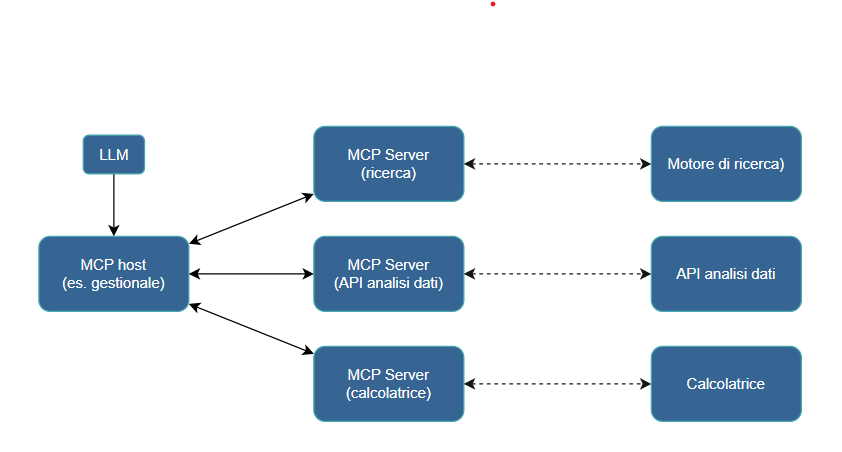
\includegraphics[alt={Schema funzionamento MCP}, height=6cm]{img/schemaMCP.png}
    \caption{Schema di funzionamento MCP}
    \label{fig:schemaMCP}
\end{figure}

La soluzione adottata si basa sulla sinergia tra \textbf{\gls{langchain}} e un protocollo custom, il \textbf{\gls{mcp}}.
\gls{langchain} è stato scelto come \gls{framework} di orchestrazione perché permette di astrarre la complessità della comunicazione con l'\gls{llm}, fornendo blocchi pre-costruiti per la gestione della memoria e per l'implementazione del ciclo Ragione-Azione (\textit{ReAct}).

A complemento, il \gls{mcp} è stato definito per disaccoppiare la logica degli strumenti dal modello specifico. Mentre le \gls{api} native (es. OpenAI Function Calling) legano l'implementazione a un singolo \textit{provider}, il \gls{mcp} definisce un contratto agnostico. Questa scelta garantisce:
\begin{itemize}
    \item \textbf{Flessibilità}: Possibilità di sostituire l'\gls{llm} sottostante senza riscrivere la logica degli strumenti.
    \item \textbf{Controllo e Sicurezza}: Centralizzazione della validazione e dell'esecuzione degli strumenti sul nostro \gls{backend}.
    \item \textbf{Estensibilità}: Semplificazione nell'aggiunta di nuovi strumenti.
\end{itemize}

% --------------------------------------------------------------------
\section{Gestione e Persistenza dei Dati}
\label{sec:data_persistence}

\subsection{Definizione del problema}
La gestione dei dati si articola su due sfide distinte: la persistenza affidabile dei dati operativi dell'applicazione (sessioni utente, conversazioni) e la gestione dei \textit{set} di dati derivati dall'analisi, che devono essere archiviati e resi disponibili per l'uso da parte dell'\gls{llm}. Le scelte in questo ambito dovevano tenere conto dell'infrastruttura tecnologica preesistente in azienda per minimizzare l'impatto operativo.

\subsection{Analisi delle alternative}
L'analisi si è concentrata su due domini: il database primario e il formato di esportazione dati.

\subsubsection{Alternative per il Database Primario}
Un \textit{database} relazionale (SQL) come \textbf{PostgreSQL} rappresentava la scelta teoricamente ottimale per garantire la massima integrità referenziale e consistenza dei dati (proprietà ACID). Tuttavia, la sua adozione avrebbe significato introdurre e manutenere un nuovo sistema nello \textit{stack} aziendale, con un conseguente \textit{overhead} operativo. L'alternativa era allinearsi alla tecnologia già in uso, ovvero un \textit{database} \gls{nosql} come \textbf{MongoDB}.

\subsubsection{Alternative per il Formato di Esportazione Dati}
\begin{itemize}
    \item \textbf{JSON/JSONL}: Formato leggibile e flessibile, ottimo per dati gerarchici, ma verboso per dati tabellari e meno diretto da importare in strumenti statistici.
    \item \textbf{Parquet o Arrow}: Formati binari colonnari ad alte \textit{performance}, ideali per \textit{Big Data}, ma illeggibili all'uomo e non immediatamente ispezionabili senza strumenti specifici.
    \item \textbf{\gls{csv}}: Formato testuale tabellare universalmente riconosciuto, semplice, leggibile e facilmente manipolabile con librerie standard.
\end{itemize}

\subsection{Soluzione adottata e motivazioni}
Le scelte sono state guidate da un criterio di pragmatismo e coerenza con il contesto aziendale.

\subsubsection{Soluzione per il Database Primario: MongoDB}
È stato adottato \textbf{MongoDB}. Sebbene altri sistemi potessero offrire vantaggi tecnici specifici, la coerenza con lo \textit{stack} aziendale è stata il criterio predominante. L'infrastruttura tecnologica di Devess si basa già su MongoDB, e questa scelta ha permesso di:
\begin{itemize}
    \item \textbf{Semplificare l'integrazione} e allinearsi alle competenze interne del \textit{team}.
    \item \textbf{Ridurre l'\textit{overhead} operativo}, evitando l'introduzione di un nuovo sistema da gestire.
\end{itemize}

\subsubsection{Soluzione per il Formato di Esportazione: \gls{csv}}
Si è optato per il formato \textbf{\gls{csv}} per la sua combinazione unica di semplicità, interoperabilità e, soprattutto, compatibilità con gli \gls{llm}. Un fattore decisivo è stata la sua \textbf{compatibilità nativa con i modelli linguistici avanzati}: modelli come Claude possono analizzare direttamente il contenuto di un file \gls{csv}, permettendo di passare un contesto dati ricco e strutturato all'\textit{agente} in modo efficiente.

\newpage
% --------------------------------------------------------------------
\section{Interfaccia Utente e Visualizzazione Dati}
\label{sec:frontend_analysis}

\subsection{Definizione del problema}
Il \gls{frontend} ha la sfida di presentare i risultati delle analisi dell'agente \gls{llm} in modo chiaro, intuitivo e interattivo. Poiché le visualizzazioni richieste dal prototipo hanno una struttura predefinita (un \textit{set} fisso di grafici popolati con dati dinamici), il problema era trovare l'architettura più snella ed efficiente per realizzare questo compito, evitando complessità non necessarie.

\subsection{Analisi delle alternative}
Sono state valutate due architetture praticabili per visualizzare dati aggiornati su \textit{dashboard} strutturalmente fisse.
\begin{itemize}
    \item \textbf{Approccio con Piattaforma Esterna (es. Grafana)}: Questa architettura prevede che il \gls{backend} salvi i dati in un \textit{database} intermedio, a cui una piattaforma come Grafana si collega per generare i grafici. Questi verrebbero poi mostrati nel \gls{frontend} tramite un componente \texttt{<iframe>}. Sebbene robusta, questa soluzione introduce una \textbf{complessità infrastrutturale significativa} (un server e un database aggiuntivi da gestire), giudicata un \textbf{onere sproporzionato} per il prototipo.
    
    \item \textbf{Altri Framework JavaScript (Vue.js, Angular)}: Pur essendo alternative valide a React, la loro adozione avrebbe introdotto una frammentazione tecnologica all'interno dello \textit{stack} di Devess, che ha standardizzato l'uso di React, andando contro la strategia aziendale.
\end{itemize}

\subsection{Soluzione adottata e motivazioni}
È stata scelta la soluzione architetturalmente più diretta: il \textbf{rendering nativo con React}. In questo flusso, il \gls{backend} invia i dati dell'analisi direttamente al \gls{frontend}, che li utilizza per popolare i componenti grafici esistenti, realizzati con librerie come Recharts.

Questa scelta è stata motivata da un'analisi pragmatica dei costi e dei benefici:
\begin{itemize}
    \item \textbf{Minima Complessità Architetturale}: L'approccio evita componenti esterni, rendendo il sistema più semplice da sviluppare, testare e distribuire.
    \item \textbf{Efficienza dei Costi e delle Risorse}: Non richiedendo servizi aggiuntivi, l'architettura minimizza i costi operativi e il carico di manutenzione.
    \item \textbf{Integrazione e Controllo Totale}: Il \textit{rendering} nativo offre un controllo completo sull'aspetto e sull'interattività dei grafici, garantendo una coerenza visiva e un'esperienza utente fluida.
\end{itemize}
In sintesi, si è scelto l'approccio che offriva il percorso più semplice ed efficiente per raggiungere l'obiettivo, incarnando il principio di evitare complessità non strettamente necessaria.